% !TeX spellcheck = it_IT
\documentclass[10pt,a4paper]{article}

\usepackage[utf8]{inputenc}
\usepackage[T1]{fontenc}	
\usepackage[italian]{babel}
\usepackage{amsmath}
\usepackage{amsfonts}
\usepackage{amssymb}
\usepackage{graphicx}

\usepackage[left=2cm,right=2cm,top=2cm,bottom=2cm]{geometry}
\geometry{a4paper}

\usepackage{booktabs} % for much better looking tables
\usepackage{verbatim}
\usepackage{subfig} % make it possible to include more than one captioned figure/table in a single 

\usepackage{fancyhdr} % This should be set AFTER setting up the page geometry
\pagestyle{fancy} % options: empty , plain , fancy
\renewcommand{\headrulewidth}{0pt} % customise the layout...
\lhead{}\chead{}\rhead{}
\lfoot{}\cfoot{\thepage}\rfoot{}

%%% SECTION TITLE APPEARANCE
\usepackage{sectsty}
%\allsectionsfont{\sffamily\mdseries\upshape} % (See the fntguide.pdf for font help)
% (This matches ConTeXt defaults)

% pacchetti che mi fanno schifo ma uso lo stesso (Bob è scemo, ma anche Ale...)
\usepackage[cdot, thickqspace, squaren]{SIunits}
% il miglior pacchetto che potessi desiderare
\usepackage{float}
% macro che mi piacciono
\def\code#1{\texttt{#1}}


\title{Esercitazione 8: Oscillatore sinusoidale a ponte di Wien con OpAmp}

\author{Gruppo BE \\ Alessandro Candido, Roberto Ribatti}
\date{\today}
\begin{document}
\maketitle

\section{Scopo e strumentazione}
Lo scopo dell'esperienza è realizzare un oscillatore ad onda sinusoidale a ponte di Wien utilizzando un OpAmp.

La strumentazione usata è quella presente sul banco di lavoro, più l'OpAmp TL081 e i diodi 1N1711.
%in realtà sia per l'OpAmp che per i diodi non abbiamo controllato che modello fossero, ce lo scriviamo comunque?
%c'è da inserire lo schema del circuito (si può anche copiare dalle slides)

\section{Loop gain del circuito}
Si è disconnesso il circuito nel punto A, connettendo l'ingresso non-invertente dell'OpAmp al generatore di funzioni e osservando con l'oscilloscopio il segnale all'altro estremo rimasto disconnesso.
Si è in questo modo misurato il loop gain (modulo e fase) per varie frequenze immesse dal generatore di funzioni. Si riportano i grafici in \figurename{~\ref{fig:Bode}} e \figurename{~\ref{fig:fasi}}, e la tabella con i dati in appendice (\tablename{~\ref{tab:loop}}).

\begin{figure}[H]
	\begin{minipage}{\textwidth}
		\centering
		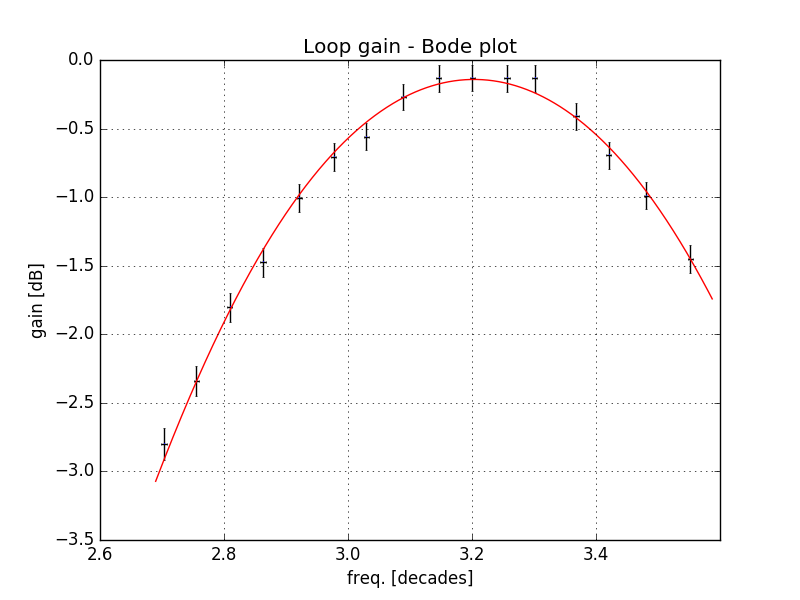
\includegraphics[width=0.8\textwidth]{../grafici/fit_loopgain_bode.pdf}
		\caption{Bode plot del guadagno di loop}
		\label{fig:Bode}
	\end{minipage}
\end{figure}

%inserire risultati dei fit, quando si è capito quali sono quelli giusti

La frequenza a cui lo sfasamento si annulla è stata misurata e il valore è $f_0 = \unit{1.80 \pm 0.05}{\kilo\hertz}$.

Si è osservato che l'ampiezza del segnale di output dipende in modo monotono dalla posizione del potenziometro. Questo è coerente con il comportamento atteso:
\begin{equation}
A = 1 + \frac{(1-f)POT_1 + R_4 + (R_3//R_{diodi})}{R_5 + f POT_1}
\label{eq:pot}
\end{equation}

In cui $f$ è la frazione di potenziometro che va verso $R_5$.

\section{Comportamento dell'output in funzione della posizione del potenziometro}
Si è riconnesso il circuito nel punto A e si è osservata la dipendenza del segnale in uscita in funzione della posizione del potenziometro.

Si è ottenuto che per alti valori di f non si osservava alcuna oscillazione, mentre al diminuire di $f$ (definito in \eqref{eq:pot}) l'ampiezza del segnale in output aumentava, fino a raggiungere la saturazione.

Questo comportamento trova riscontro con quanto atteso: infatti la condizione di Barkhausen impone come conseguenza che $A = 3$. Per ottenere questo valore dato un certo $f$ quello che varia è la resistenza dinamica dei diodi, e quindi il punto di lavoro (si confronti l'equazione \eqref{eq:pot}).

Per cui, imponendo che $R_3 = R_4 = R_5 = POT_1 = \unit{10}{\kilo\ohm}$ si ottiene dalla \eqref{eq:pot}:
\begin{equation}
A = 1 + \frac{2 - f + (1 + 10k/R_{diodi})^{-1}}{1+f}
\end{equation}

Per cui per avere $A = 3$ con $f \sim 1$ si dovrebbe avere $(1 + 10k/R_{diodi})^{-1} \sim 3$, che è impossibile poiché il primo membro è sempre $\leq 1$.
Per $f$ più piccoli si riduce il valore richiesto per $(1 + 10k/R_{diodi})^{-1}$, infatti per $f = 1/3$ si ottiene che $(1 + 10k/R_{diodi})^{-1} = 1$, e questo è possibile per valori di $R_{diodi}$ molto elevati. Man mano che decresce $f$ decresce dunque il valore richiesto della resistenza dinamica, spostando il punto di lavoro a tensioni di output maggiori, fino ad arrivare a $f = 0 \implies (1 + 10k/R_{diodi})^{-1} = 0 \implies R_{diodi} = 0$ per cui uno dei diodi deve essere completamente in conduzione (in pratica dovrebbe essere un cortocircuito).

Per valori così piccoli di $f$ si porta l'output a saturazione, e quindi viene distorto, come mostrato nell'immagine a destra in \figurename{~\ref{fig:dippot}}, mentre nell'immagine a sinistra è mostrato il funzionamento in regime lineare, per cui l'uscita è una sinusoide e la tensione picco-picco è minore di quella nell'altra immagine.

\begin{figure}[H]
    \centering
    \begin{minipage}{0.49\textwidth}
	    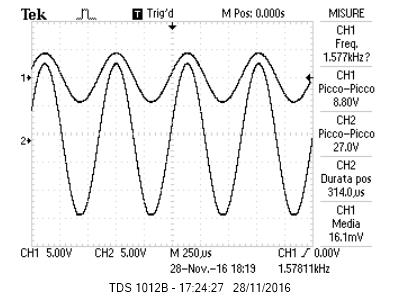
\includegraphics[width=\textwidth]{../oscilloscopio/punto5.jpg}
    \end{minipage}
    \begin{minipage}{0.49\textwidth}
        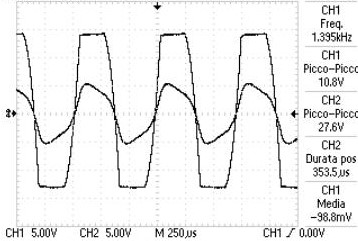
\includegraphics[width=\textwidth]{../oscilloscopio/punto5(scazzo).jpg}
    \end{minipage}
    \caption{Dipendenza del segnale in uscita dalla posizione del potenziometro}
    \label{fig:dippot}
\end{figure}

\section{Frequenza di oscillazione}
La frequenza di oscillazione misurata è pari a $\unit{1.57 \pm 0.02}{\kilo\hertz}$.
% in questa sezione manca il confronto con la teoria, te lo lascio.

\subsection{Dipendenza dalla posizione del potenziometro}
La frequenza di oscillazione osservata è risultata indipendente dalla posizione del potenziometro.

\subsection{Dipendenza dalla tensione di alimentazione}
La frequenza di oscillazione risulta indipendente dalla tensione di alimentazione, fintanto che questa non diventi abbastanza ridotta da portare il segnale di output in clipping.

\section{Guadagno all'innesco dell'oscillazione}

Ci si è posti alla posizione del potenziometro corrispondente all'innesco dell'oscillazione e si sono misurati i seguenti valori per le tensioni:

\begin{table}[H]
	\centering
	\begin{tabular}{cc}
        $ V_+ = \unit{256 \pm 8}{\milli\volt}$  & $V_{out} = \unit{820 \pm 26}{\milli\volt}$
	\end{tabular}
\end{table}

Da cui si ricava un guadagno $A = 3.20 \pm 0.14$ che è compatibile con 3 a poco più di $1\sigma$.

\section{Scopo dei diodi}
Lo scopo dei diodi è di inserire un elemento non lineare nella rete di amplificazione, in modo da stabilizzare la tensione sull'output.

Infatti se il potenziometro viene ruotato l'amplificazione dovuta alla rete costituita dalle resistenze $R_5, R_4, R_3$, i diodi, l'OpAmp e il potenziometro stesso cambia, e in risposta cambia il punto di lavoro dei diodi, impedendo al guadagno di modificarsi eccessivamente.

In particolare, con riferimento all'equazione \eqref{eq:pot}:
\begin{description}
\item[aumenta $f$] diminuirebbe il guadagno $A$, ma allora la resistenza dinamica dei diodi tenderebbe ad aumentare, mantenendo quindi $A$ alto;
\item[diminuisce $f$] aumenterebbe il guadagno $A$, ma in questo caso i diodi andrebbero sempre più in conduzione, diminuendo quindi il guadagno $A$, cioè stabilizzandolo.
\end{description}

I diodi quindi svolgono il ruolo di feedback negativo sul guadagno $A$, cioè lo mantengono stabile rispetto alle variazioni di altri elementi, rendendo quindi possibile lavorare in regime lineare con un intervallo maggiore di valori.

In assenza di diodi, invece, si perde stabilità, e provando a ruotare il potenziometro si passa da un regime in cui non vi sono oscillazioni a un regime in cui le oscillazioni vanno in saturazione.

In \figurename{~\ref{fig:wdiod}} si osserva nell'immagine di sinistra che anche al limite minimo per cui compaiono le oscillazioni vanno in saturazione (come si vede in basso su \code{CH2}), mentre nell'immagine di destra si ha un esempio più evidente di saturazione.

\begin{figure}[H]
    \centering
    \begin{minipage}{0.49\textwidth}
	    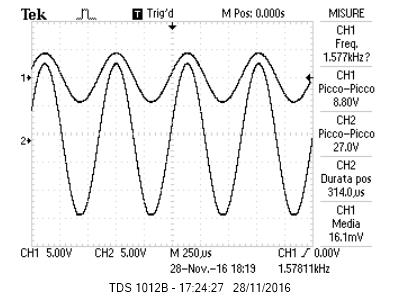
\includegraphics[width=\textwidth]{../oscilloscopio/punto5.jpg}
    \end{minipage}
    \begin{minipage}{0.49\textwidth}
        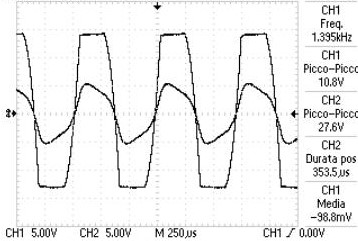
\includegraphics[width=\textwidth]{../oscilloscopio/punto5(scazzo).jpg}
    \end{minipage}
    \caption{Risposta del circuito in assenza di diodi}
    \label{fig:wdiod}
\end{figure}

\pagebreak
\section{Appendice: Dati acquisiti}
Si riportano qui le tabelle dei dati usati per i fit e i grafici.
\centering
\begin{figure}[H]
	\centering
	\resizebox{0.7\textwidth}{!}{
	\input{../tabelle/tab_loopgain.txt}}
	\captionof{table}{Loopgain}
	\label{tab:loop}
\end{figure}

\end{document}
